\documentclass[twoside,14pt,openany,letterpaper]{memoir}%
\usepackage[T1]{fontenc}%
\usepackage[utf8]{inputenc}%
\usepackage{lmodern}%
\usepackage{textcomp}%
\usepackage{lastpage}%
%
\usepackage[noprint,1to1]{booklet}%
\usepackage{titlesec}%
\titleformat{\chapter}[display]%
{\normalfont\bfseries}{}{0pt}{\Huge}%
\usepackage{pdfpages}%
\usepackage{hyperref}%
\usepackage{graphicx}%
\graphicspath{ {resources/} }%

\setulmarginsandblock{1.65cm}{1.65cm}{*}%
\setlrmarginsandblock{1cm}{1cm}{*}%
\checkandfixthelayout%

\renewcommand{\thesection}{\arabic{section}}%
\title{Passover Songs}%
\author{compiled by Maia McCormick}%
\date{\today}%
%
\begin{document}%
\normalsize%
% \newcommand{\invisiblesection}[1]{\refstepcounter{section}\sectionmark{#1}\addcontentsline{toc}{section}{#1}}%
\newcommand\song[2]{
  \chapter[#1 {\itshape#2}]{#1 \Large\itshape#2}
}
\newcommand\translation[1]{
	\vspace*{\fill}
	\large\textbf{TRANSLATION:\\}
	\normalsize\textit{#1}
}

\pagenumbering{gobble}%
\maketitle%

\begin{figure}[h]
\vspace{3.0cm}
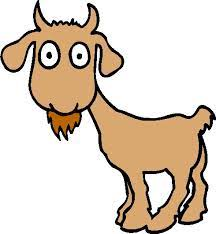
\includegraphics[scale=0.5]{coverImg}
\centering
\end{figure}

\clearpage%
\tableofcontents%
\clearpage%
\pagenumbering{arabic}%

% TODO:
% - Eliahu

% CHAD GADYA %
\song{Chad Gadya (One Little Kid)}{trad.}
Chad gadya, chad gadya.\\
\\
That my father bought for two zuzim, chad gadya, chad gadya.\\
\\
Then came the cat that ate the kid\\
that my father bought for two zuzim,\\
chad gadya, chad gadya.\\
\\
Then came the dog that bit the cat...\\
Then came the stick that beat the dog...\\
Then came the fire that burnt the stick...\\
Then came the water that quenched the fire...\\
Then came the ox that drank the water...\\
Then came the butcher that slaughtered the ox...\\
Then came the Angel of Death that killed the butcher...\\
Then came the Holy One, Blessed be He that slew the the Angel of Death\\
\indent that killed the butcher\\
\indent that slaughtered the ox\\
\indent that drank the water\\
\indent that quenched the fire\\
\indent that burnt the stick\\
\indent that beat the dog\\
\indent that bit the cat\\
\indent that ate the kid\\
\indent that my father bought for two zuzim,\\
\indent chad gadya, chad gadya.\\

% DAYENU %
\song{Dayenu (It Would Have Been Enough)}{trad.}
Ilu hotzi- hotzianu,\\
hotzianu mimitzrayim,\\
hotzianu mimitzrayim, dayenu!\\
\\
\footnotesize{CHORUS:}\normalsize\\
Day-dayenu, day-dayenu,\\
day-dayenu, dayenu dayenu!\\
\\
Ilu natan, natan lanu\\
natan lanu et hashabbat,\\
natan lanu et hashabbat, dayenu!\\
\\
Ilu natan, natan lanu\\
natan lanu et hatorah,\\
natan lanu et hatorah, dayenu!\\

\translation{
	If He had only brought us out from Egypt...\\
	If He had only given us the Shabbat...\\
	If He had only given us the Torah...\\
  \\
	It would have been enough!\\
}

% HAVA NASHIRA %
\song{Hava Nashira}{mel. Johannes Ockeghem}
Hava nashira, shir’ haleluyah (3x)

\begin{figure}[h]
\vspace{3.0cm}
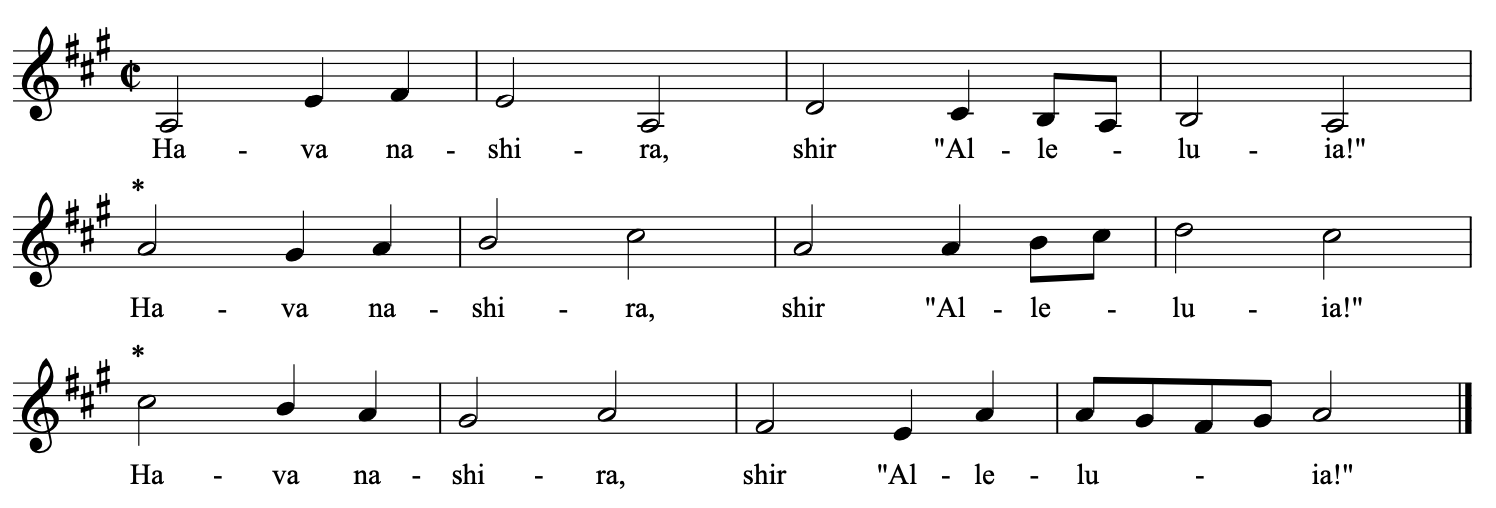
\includegraphics[scale=0.75]{havaNashira}
\centering
\end{figure}

\translation{Let us sing together, sing Halleluyah!}

% MAH NISHTANA %
\song{Mah Nishtana (The Four Questions)}{trad.}
Mah Nishtana halayla hazeh mikol haleylot? Mikol haleylot?\\
\\
Sheb-ch-ol haleylot anu o-ch-lim ch-ametz umatzah,\\
ch-ametz umatzah.\\
Halaylah hazeh, halaylah hazeh kulo matzah (2x)\\
\\
Sheb-ch-ol haleylot anu o-ch-lim she-ar yerakot,\\
she-ar yerakot.\\
Halayla hazeh, halayla hazeh maror (2x)\\
\\
Sheb-ch-ol haleylot eyn anu matbilin afilu pa-am e-ch-at,\\
filu pa-am e-ch-at.\\
Halayla hazeh, halayla hazeh sh’tae p’amim (2x)\\
\\
Sheb-ch-ol haleylot anu o-ch-lim beyn yoshvin uveyn mesubin,\\
beyn yoshvin uveyn mesubin.\\
Halayla hazeh, halayla hazeh kulanu mesubin (2x)\\

\translation{
	What makes this night different from all [other] nights?\\
	On all nights we need not dip even once; on this night we do so twice.\\
	On all nights we eat chametz or matzah; on this night only matzah.\\
	On all nights we eat any kind of vegetables; on this night maror.\\
	On all nights we eat sitting upright or reclining; on this night we all recline.\\
}

% MIRIAM'S SONG %
\song{Miriam's Song}{by Debbie Friedman}

And the women dancing with their timbrels\\
Followed Miriam as she sang her song\\
Sing a song to the One whom we’ve exalted\\
Miriam and the women danced and danced the whole night long.\\
\\
And Miriam was a weaver of unique variety\\
The tapestry she wove was one which sang our history\\
With every strand and every thread she crafted her delight\\
A woman touched with spirit, she dances toward the light.\\
\\
When Miriam stood upon the shores and gazed across the sea\\
The wonder of this miracle she soon came to believe\\
Whoever thought the sea would part with an outstretched hand\\
And we would pass to freedom and march to the promised land.\\
\\
And Miriam the prophet took her timbrel in her hand\\
And all the women followed her just as she had planned\\
And Miriam raised her voice in song, she sang with praise and might:\\
"We’ve just lived through a miracle; we’re going to dance tonight!"\\

\clearpage%
\printindex%
\end{document}
